\chapter{Supporting figures of the wavelet analysis and momentum flux calculation in Chapter \ref{sec:results3D}}
\label{appA}
\thispagestyle{plain}
%
\begin{figure*}[tbp]
    \centering
    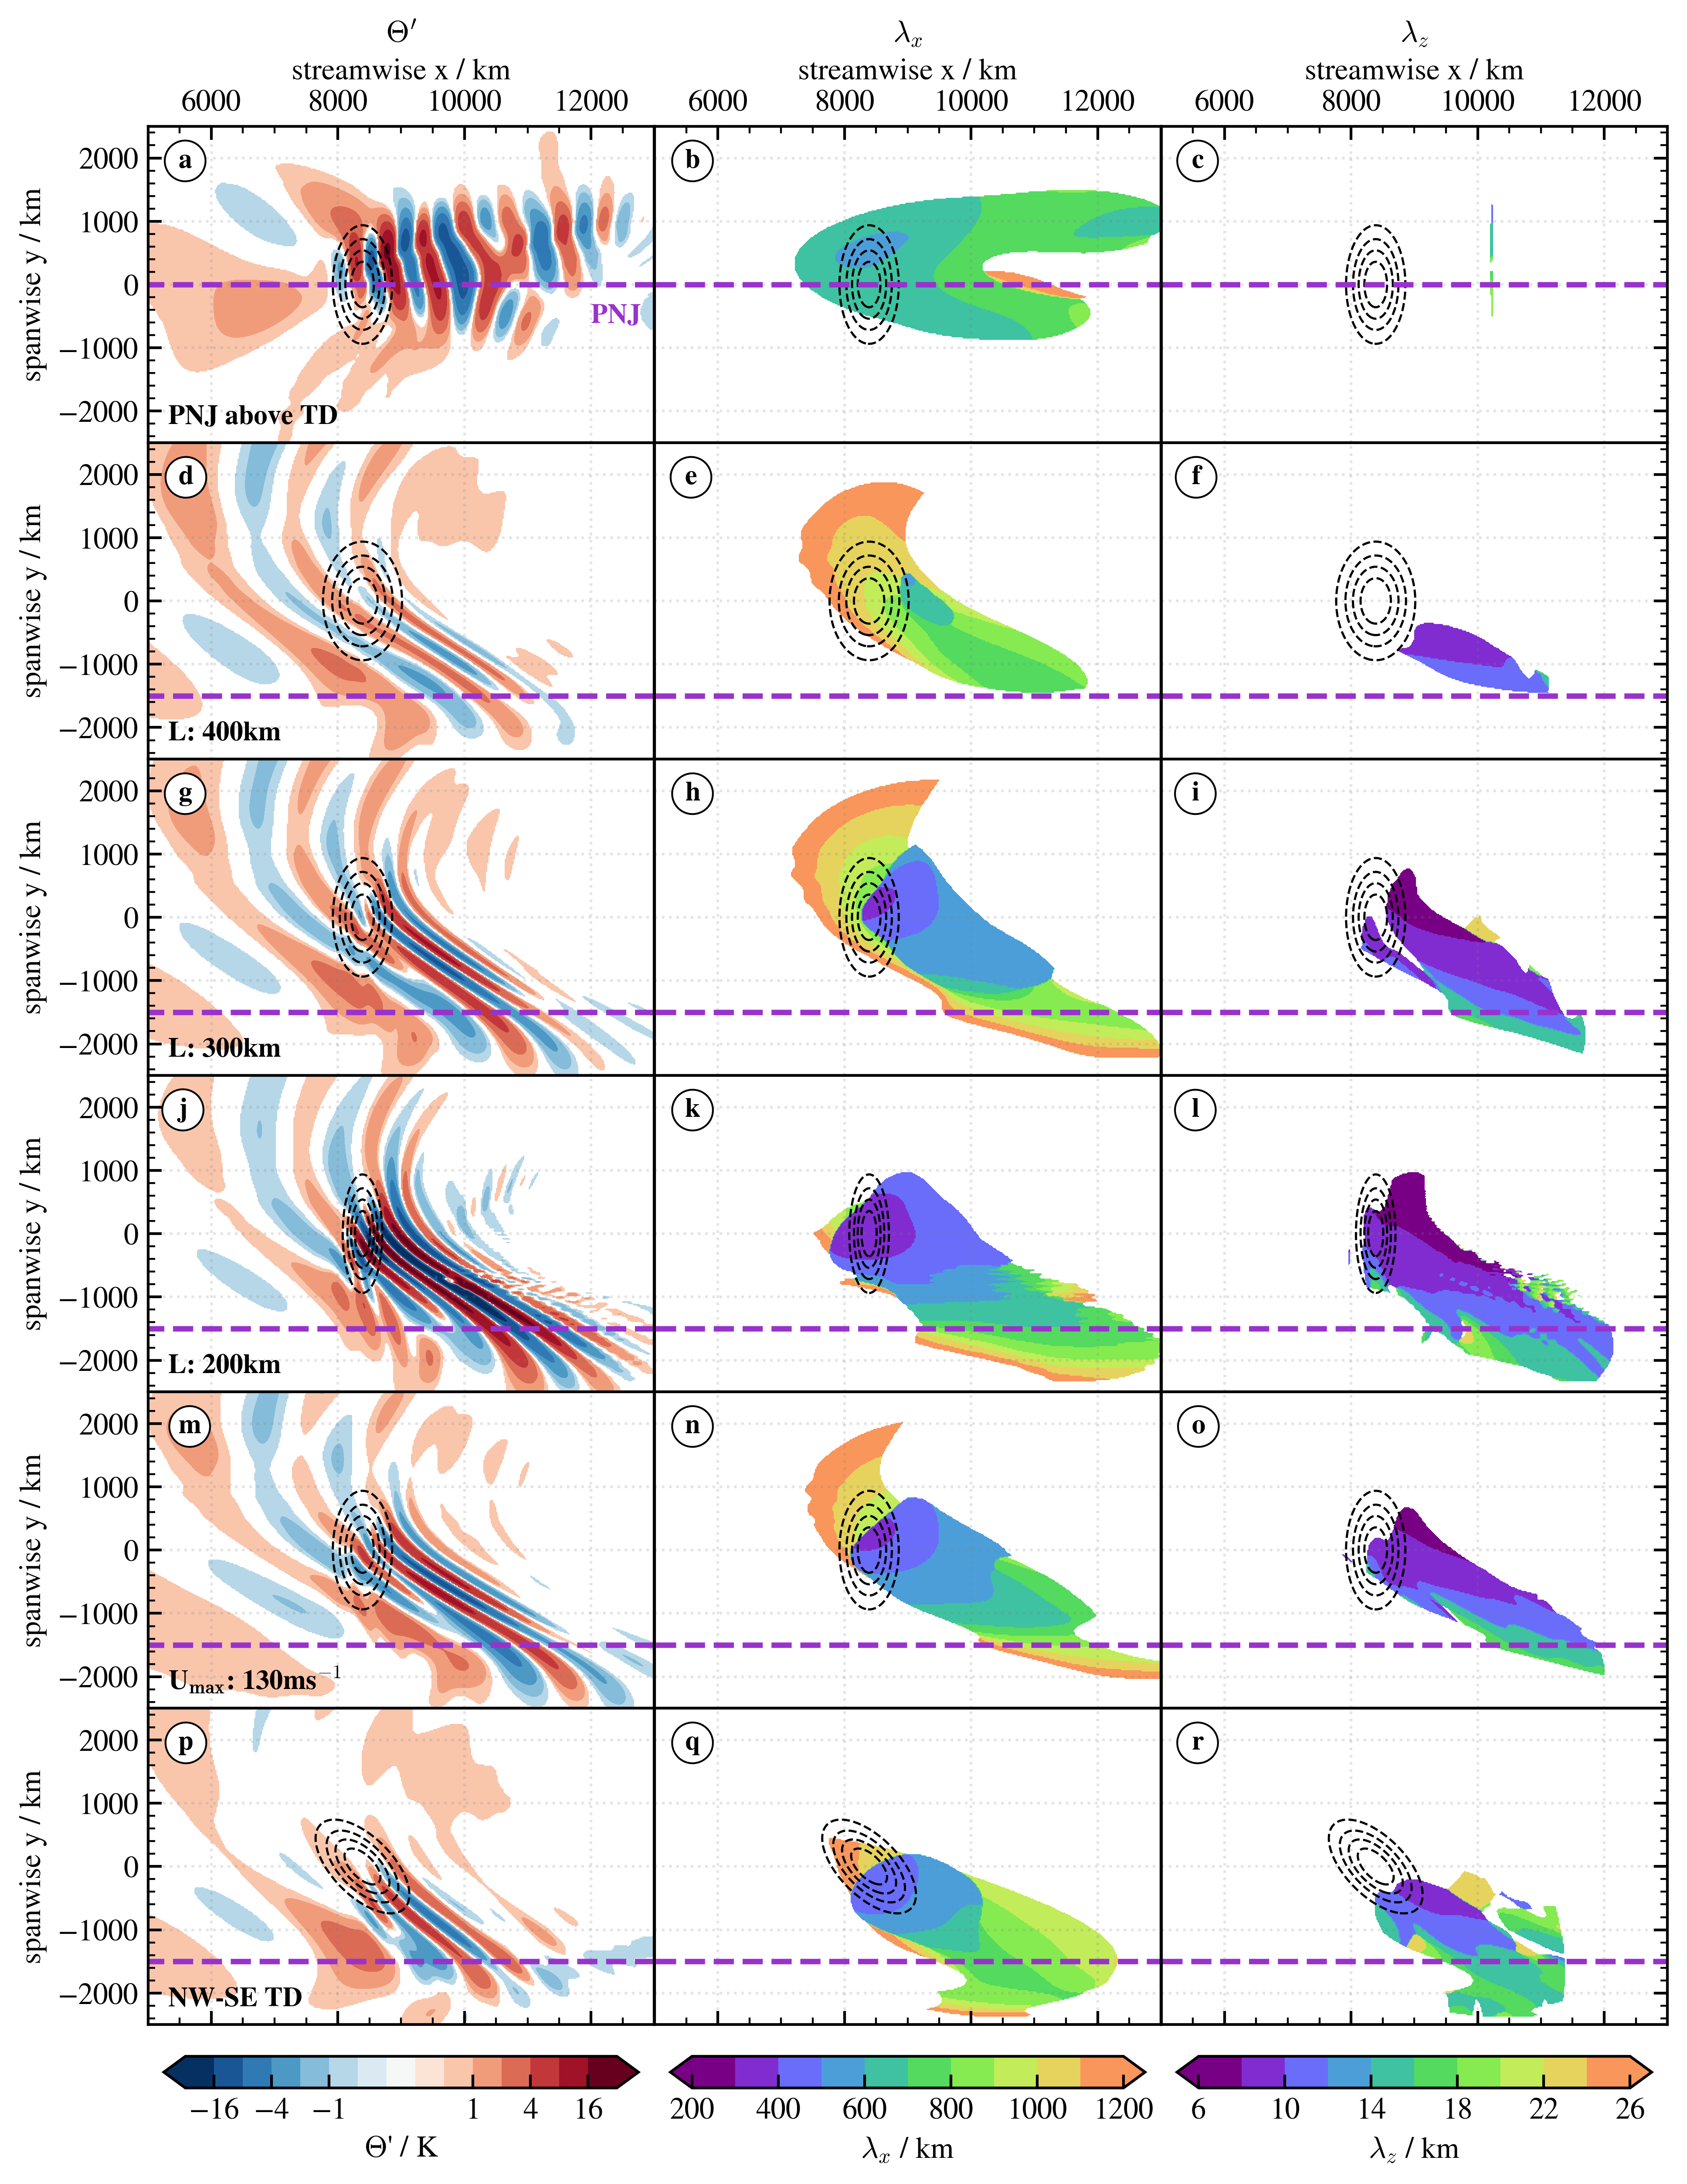
\includegraphics[width=0.99\textwidth]{figures_3D/waveletAna_overview.png}
    \caption{Similar cross sections as Figure \ref{fig:waveletAna}, but showing the zonal wavelength $\lambda_x$ in the second column and vertical wavelength $\lambda_z$ in the third column. The wavelenghts are based on a 1D wavelet analysis in each dimension.}
    \label{fig:waveletAna_xz}
\end{figure*}
%
\begin{figure*}[tbp]
    \centering
    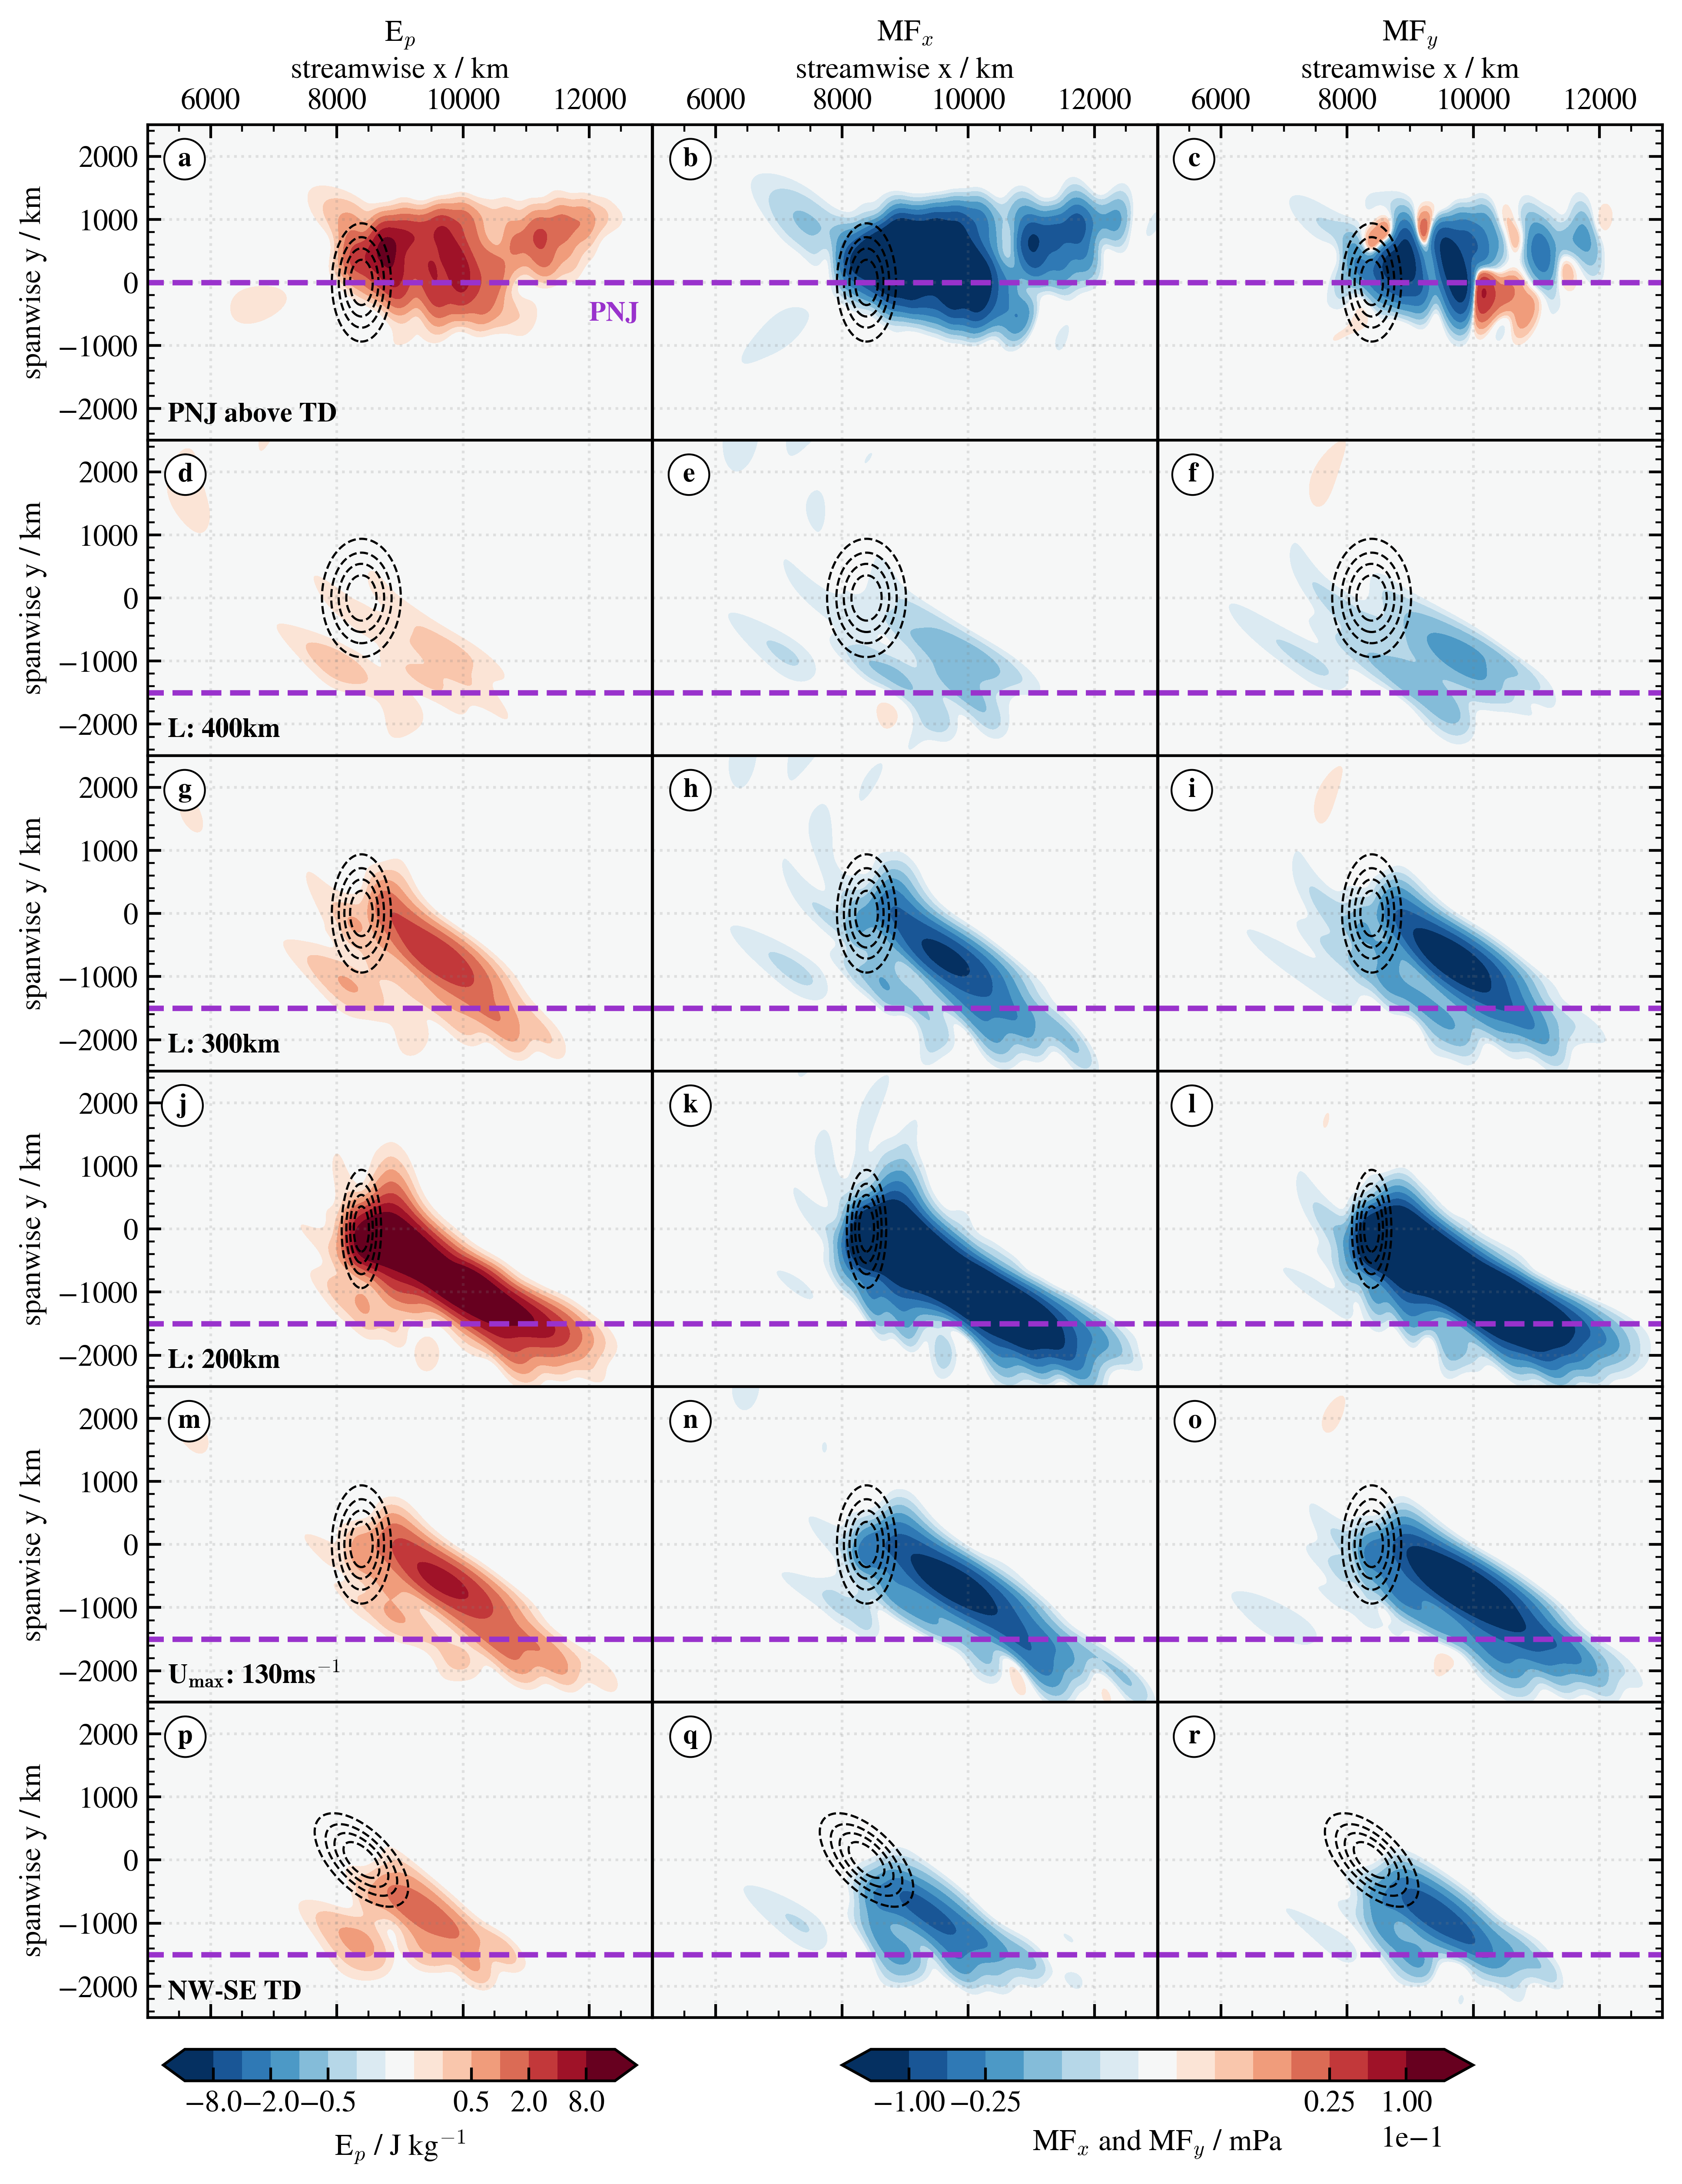
\includegraphics[width=0.99\textwidth]{figures_3D/waveletAna_mf.png}
    \caption{Similar cross sections as Figure \ref{fig:waveletAna}, but showing the potential energy E$_p$ in the first column, the zonal momentum flux MF$_x= \bar{\rho} \overbar{u'w'}$ in the second column and meridional momentum flux MF$_y= \bar{\rho} \overbar{v'w'}$ in the third column.}
    \label{fig:waveletAna_mf}
\end{figure*}
%
% Large quantities of data should be placed in an appendix. They should only be ``summarized'' in the chapter Results. Another way is to present some representative cases together with some extreme cases in the chapter Results. In any case, there should always appear a reference to the appendix in the main part of the thesis.